% Тип документа
\documentclass[a4paper,12pt]{extarticle}

% Шрифты, кодировки, символьные таблицы, переносы
\usepackage{cmap}
\usepackage[T2A]{fontenc}
\usepackage[utf8x]{inputenc}
\usepackage[russian]{babel}

% Это пакет -- хитрый пакет, он нужен но не нужен
\usepackage[mode=buildnew]{standalone}

\usepackage
	{
		% Дополнения Американского математического общества (AMS)
		amssymb,
		amsfonts,
		amsmath,
		amsthm,
		% misccorr,
		% 
		% Графики и рисунки
		wrapfig,
		graphicx,
		subcaption,
		float,
		tikz,
		tikz-3dplot,
		caption,
		csvsimple,
		color,
		booktabs,
		pgfplots,
		pgfplotstable,
		geometry,
		% 
		% Таблицы, списки
		makecell,
		multirow,
		indentfirst,
		%
		% Интегралы и прочие обозначения
		ulem,
		esint,
		esdiff,
		% 
		% Колонтитулы
		fancyhdr,
	}  


% Обводка текста в TikZ
\usepackage[outline]{contour}

% Увеличенный межстрочный интервал, французские пробелы
\linespread{1.3} 
\frenchspacing 

 
\usetikzlibrary
	{
		decorations.pathreplacing,
		decorations.pathmorphing,
		patterns,
		calc,
		scopes,
		arrows,
		fadings,
		through,
		shapes.misc,
		arrows.meta,
		3d,
		quotes,
		angles,
		babel
	}


\tikzset{
	force/.style=	{
		>=latex,
		draw=blue,
		fill=blue,
				 	}, 
	%				 	
	axis/.style=	{
		densely dashed,
		blue,
		line width=1pt,
		font=\small,
					},
	%
	th/.style=	{
		line width=1pt},
	%
	acceleration/.style={
		>=open triangle 60,
		draw=magenta,
		fill=magenta,
					},
	%
	inforce/.style=	{
		force,
		double equal sign distance=2pt,
					},
	%
	interface/.style={
		pattern = north east lines, 
		draw    = none, 
		pattern color=gray!60,
					},
	cross/.style=	{
		cross out, 
		draw=black, 
		minimum size=2*(#1-\pgflinewidth), 
		inner sep=0pt, outer sep=0pt,
					},
	%
	cargo/.style=	{
		rectangle, 
		fill=black!70, 
		inner sep=2.5mm,
					},
	%
	caption/.style= {
		midway,
		fill=white!20, 
		opacity=0.9
					},
	%
	}

\newenvironment{tikzpict}
    {
	    \begin{figure}[htbp]
		\centering
		\begin{tikzpicture}
    }
    { 
		\end{tikzpicture}
		% \caption{caption}
		% \label{fig:label}
		\end{figure}
    }


\newcommand{\vbLabel}[3]{\draw ($(#1,#2)+(0,5pt)$) -- ($(#1,#2)-(0,5pt)$) node[below]{#3}}
\newcommand{\vaLabel}[3]{\draw ($(#1,#2)+(0,5pt)$) node[above]{#3} -- ($(#1,#2)-(0,5pt)$) }

\newcommand{\hrLabel}[3]{\draw ($(#1,#2)+(5pt,0)$) -- ($(#1,#2)-(5pt,0)$) node[right, xshift=1em]{#3}}
\newcommand{\hlLabel}[3]{\draw ($(#1,#2)+(5pt,0)$) node[left, xshift=-1em]{#3} -- ($(#1,#2)-(5pt,0)$) }



\newcommand\zi{^{\,*}_i}
\newcommand\sumn{\sum_{i=1}^{N}}

\tikzset{
	coordsys/.style={scale=1.8,x={(1.1cm,-0cm)},y={(0.5cm,1cm)}, z={(0cm,0.8cm)}},
	coordsys/.style={scale=1.5,x={(0cm,0cm)},y={(1cm,0cm)}, z={(0cm,1cm)}}, 
	coordsys/.style={scale=1.5,x={(1cm,0cm)},y={(0cm,1cm)}, z={(0cm,0cm)}}, 
}

\usepgfplotslibrary{units}


% Draw line annotation
% Input:
%   #1 Line offset (optional)
%   #2 Line angle
%   #3 Line length
%   #5 Line label
% Example:
%   \lineann[1]{30}{2}{$L_1$}

\newcommand{\lineann}[4][0.5]{%
    \begin{scope}[rotate=#2, blue,inner sep=2pt, ]
        \draw[dashed, blue!40] (0,0) -- +(0,#1)
            node [coordinate, near end] (a) {};
        \draw[dashed, blue!40] (#3,0) -- +(0,#1)
            node [coordinate, near end] (b) {};
        \draw[|<->|] (a) -- node[fill=white, scale=0.8] {#4} (b);
    \end{scope}
}

\newcommand{\lineannn}[4][0.5]{%
    \begin{scope}[rotate=#2, blue,inner sep=2pt, ]
        \draw[dashed, blue!40] (0,0) -- +(0,#1)
            node [coordinate, near end] (a) {};
        \draw[dashed, blue!40] (#3,0) -- +(0,#1)
            node [coordinate, near end] (b) {};
        % \draw[color=white, color=blue] (a) -- node[fill=white, scale=0.8] {#4} (b);
        \draw[->|] (a)++(-0.3,0) -- (a);
        \draw[->|] (b)++(0.3,0) coordinate (xx) -- (b);
        \draw (xx) node[fill=white, scale=0.8, right] {#4};
    \end{scope}
}

% Круговая стрелка относительно центра (дуга из центра)
\tikzset{
  pics/carc/.style args={#1:#2:#3}{
    code={
      \draw[pic actions] (#1:#3) arc(#1:#2:#3);
    }
  },
  dash/.style={
  	dash pattern=on 5mm off 5mm
  }
}

% Среднее <#1>
\newcommand{\mean}[1]{\langle#1\rangle}

\pgfplotsset{
    % most recent feature set of pgfplots
    compat=newest,
}

% const прямым шрифтом
\newcommand\ct[1]{\text{\rmfamily\upshape #1}}
\newcommand*{\const}{\ct{const}}


\usepackage[europeanresistors,americaninductors]{circuitikz}

% Style to select only points from #1 to #2 (inclusive)
\pgfplotsset{select/.style 2 args={
    x filter/.code={
        \ifnum\coordindex<#1\def\pgfmathresult{}\fi
        \ifnum\coordindex>#2\def\pgfmathresult{}\fi
    }
}}


\usepackage{array}



%%%%%%%%%%%%%%%%%%%%%%%%%%%%%%%%%%%%%%%%%%%%%%%%%
\makeatletter
\newif\if@gather@prefix 
\preto\place@tag@gather{% 
  \if@gather@prefix\iftagsleft@ 
    \kern-\gdisplaywidth@ 
    \rlap{\gather@prefix}% 
    \kern\gdisplaywidth@ 
  \fi\fi 
} 
\appto\place@tag@gather{% 
  \if@gather@prefix\iftagsleft@\else 
    \kern-\displaywidth 
    \rlap{\gather@prefix}% 
    \kern\displaywidth 
  \fi\fi 
  \global\@gather@prefixfalse 
} 
\preto\place@tag{% 
  \if@gather@prefix\iftagsleft@ 
    \kern-\gdisplaywidth@ 
    \rlap{\gather@prefix}% 
    \kern\displaywidth@ 
  \fi\fi 
} 
\appto\place@tag{% 
  \if@gather@prefix\iftagsleft@\else 
    \kern-\displaywidth 
    \rlap{\gather@prefix}% 
    \kern\displaywidth 
  \fi\fi 
  \global\@gather@prefixfalse 
} 
\newcommand*{\beforetext}[1]{% 
  \ifmeasuring@\else
  \gdef\gather@prefix{#1}% 
  \global\@gather@prefixtrue 
  \fi
} 
\makeatother
%%%%%%%%%%%%%%%%%%%%%%%%%%%%%%%%%%%%%%%%%%%%%%%%%

\geometry		
	{
		left			=	2cm,
		right 			=	2cm,
		top 			=	3cm,
		bottom 			=	3cm,
		bindingoffset	=	0cm
	}

%%%%%%%%%%%%%%%%%%%%%%%%%%%%%%%%%%%%%%%%%%%%%%%%%%%%%%%%%%%%%%%%%%%%%%%%%%%%%%%

\def\labauthors{Понур К.А., Сарафанов Ф.Г., Сидоров Д.А.}
\def\labgroup{420}
\def\labnumber{222}
\def\labtheme{Изучение разряда неоновой лампы}

	%применим колонтитул к стилю страницы
\pagestyle{fancy} 
	%очистим "шапку" страницы
\fancyhead{} 
	%слева сверху на четных и справа на нечетных
\fancyhead[R]{\labauthors} 
	%справа сверху на четных и слева на нечетных
\fancyhead[L]{Отчёт по лабораторной работе №\labnumber} 
	%очистим "подвал" страницы
\fancyfoot{} 
	% номер страницы в нижнем колинтуле в центре
\fancyfoot[C]{\thepage} 

%%%%%%%%%%%%%%%%%%%%%%%%%%%%%%%%%%%%%%%%%%%%%%%%%%%%%%%%%%%%%%%%%%%%%%%%%%%%%%%

\renewcommand{\contentsname}{Оглавление}

\usepackage{tocloft}
% \renewcommand{\cftpartleader}{\cftdotfill{\cftdotsep}} % for parts
% \renewcommand{\cftsectiondotsep}{\cftdotsep}% Chapters should use dots in ToC
\renewcommand{\cftsecleader}{\cftdotfill{\cftdotsep}}
%\renewcommand{\cftsecleader}{\cftdotfill{\cftdotsep}} % for sections, if you really want! (It is default in report and book class (So you may not need it).
% ---------
% \newcommand{\cftchapaftersnum}{.}%
% \usepackage{titlesec}
% \titlelabel{\thetitle.\quad}
\usepackage{secdot}
\sectiondot{subsection}

\begin{document}

\begin{titlepage}

\begin{center}

{\small\textsc{Нижегородский государственный университет имени Н.\,И. Лобачевского}}
\vskip 1pt \hrule \vskip 3pt
{\small\textsc{Радиофизический факультет}}

\vfill

{\Large Отчет по лабораторной работе №\labnumber\vskip 12pt\bfseries \labtheme}
	
\end{center}

\vfill
	
\begin{flushright}
	{Выполнили студенты \labgroup\ группы\\ \labauthors}%\vskip 12pt Принял:\\ Менсов С.\,Н.}
\end{flushright}
	
\vfill
	
\begin{center}
	Нижний Новгород, \the\year
\end{center}

\end{titlepage}



\tableofcontents
\newpage

\section*{Введение}
\addcontentsline{toc}{section}{Введение}
\label{sec:input}

Целью данной работы является успешная сдача зачета по общефизу

\newpage
\section{Исследование неоновой лампы}
\subsection{Снятие ВАХ неоновой лампы}

\begin{table}[H]
	    \caption{Снятие вольт-амперной характеристики (ВАХ) неоновой лампы}
	    \label{tab:diod}
	    \pgfkeys{/pgf/number format/.cd,
		fixed,  1000 sep={\,}}
\newlength\Colsep
\setlength\Colsep{10pt}
\pgfplotstableset{
	multicolumn names, % allows to have multicolumn names
	col sep=tab, % the seperator in our .csv file
	precision=3,
	% fixed zerofill, 
	columns/u/.style={
	column name={$U$, В},
	},
	columns/i/.style={
	column name={$I$, мА},
	},
	empty cells with={\textbf{--}},
	every head row/.style={
	before row={\toprule},
	after row={
		\midrule}
		},
	every last row/.style={after row=\bottomrule},
	every row/.style={after row=\midrule}, 
	columns={u,i},		
	dec sep align,
	% dec zerofill
	% fixed,fixed zerofill,
	% precision=2
	}
\noindent\begin{minipage}[t][][t]{\textwidth}
\begin{minipage}[t][][b]{0.2\textwidth}
	    \pgfplotstabletypeset[
		% skip rows between index={0}{50},
		skip rows between index={25}{500},
	    ]{data/vax.csv}
\end{minipage}%\hfill
\begin{minipage}[t][][b]{0.2\textwidth}
	    \pgfplotstabletypeset[
			skip rows between index={0}{25},
			skip rows between index={50}{500},
	    ]{data/vax.csv}
\end{minipage}%
\begin{minipage}[t][][b]{0.2\textwidth}
	    \pgfplotstabletypeset[
			skip rows between index={0}{50},
			skip rows between index={75}{500},
	    ]{data/vax.csv}
\end{minipage}%
\begin{minipage}[t][][b]{0.2\textwidth}
	    \pgfplotstabletypeset[
			skip rows between index={0}{75},
			skip rows between index={100}{500},
	    ]{data/vax.csv}
\end{minipage}%
\begin{minipage}[t][][b]{0.2\textwidth}
	    \pgfplotstabletypeset[
			skip rows between index={0}{100},
			skip rows between index={125}{500},
	    ]{data/vax.csv}
\end{minipage}%
\end{minipage}		

\end{table}

\newpage

\begin{figure}[H]
	\centering
	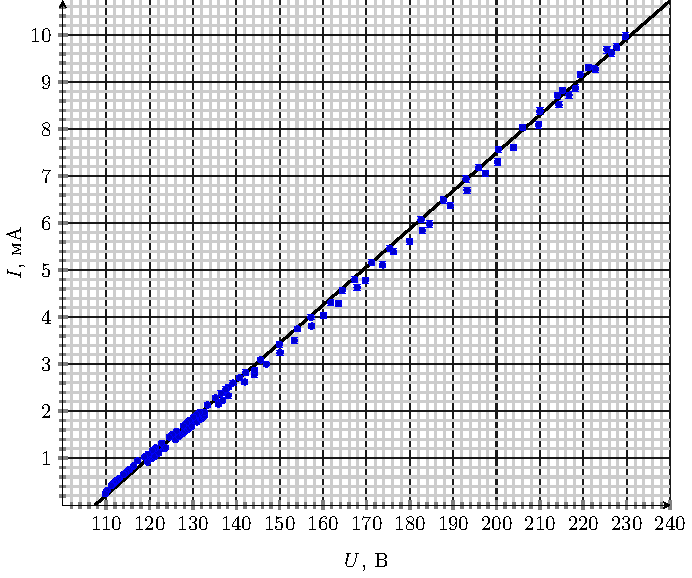
\includegraphics[width=\textwidth]{vax}
	\caption{Ход вольт-амперной характеристики неоновой лампы}
	\label{fig:figure1}
\end{figure}

Идеальная ВАХ системы из последовательно соединенных неоновой лампы и резистора
\begin{equation}
	I=\frac{U-U_0}{R_0},
\end{equation}
где по результатам аппроксимации с помощью MATLAB найдены коэффициенты 
\begin{equation}
	U_0=(107\pm1) \text{ В}
\end{equation}
\begin{equation}
	R_0=(12.36\pm0.09) \text{ кОм}
\end{equation}
<<<<<<< HEAD
\newpage
\section{Вывод формул}
Рассчитаем период колебаний генератора, схема которого представлена на рисунке.
\begin{equation}
\label{eq:1}
	\diff{U}{t}+I(V)=\frac{\mathcal{E}-U}{R} \text{, где I(U)- ток в лампе}
\end{equation}
 
\begin{center}
\Large Фёдор, как вставлять рисунки?
\end{center}

Рассмотрим стационарный режим (напряжение U на конденсаторе постоянно). 
 Сила тока в таком случае определяется уравнением
\begin{equation}
\label{eq:2}
I_{\text{ст}}=\frac{\mathcal{E}-U}{R}
\end{equation}
%график бы сюда вставить из методички
Стационарный режим работы схемы определяется путём совместного решения уравнения (\ref{eq:2}) и уравнения $I=I(U)$, описывающего ВАХ лампы. Очевидно, что точка пересечения существует не при всех R. Случай, когда

\begin{center}
$R=R_{\text{кр}}=\frac{\mathcal{E}-U}{I_{\text{г}}}$
\end{center}

является критическим, при дальнейшем увеличении сопротивления R стационарный режим оказывается невозможным.
Именно в этом случае $(R>R_{\text{кр}})$ в системе устанавливаются колебания.

%текст из методички

Рассмотрим, как происходит колебательный процесс. Пусть вначале конденсатор не заряжен. При включении схемы он начнет заряжаться через сопротивление R, напряжение U при этом будет увеличиваться. Как только оно достигнет напряжения зажигания $U_{\text{з}}$, газ в лампе начнет проводить ток, причем прохождение тока через лампу сопровождается разрядкой конденсатора. Действительно, нагрузочная прямая в этом случае не пересекается с характеристикой лампы, и значит, батарея $\mathcal{E}$, включенная через сопротивление R, не может поддерживать необходимую для горения лампы величину тока. Пока лампа горит, конденсатор разряжается, и напряжение на нем падает. Когда оно достигнет напряжения гашения $U_{\text{г}}$, лампа перестанет проводить ток, и конденсатор вновь начнет заряжаться. Очевидно, амплитуда колебаний равна $U_{\text{з}}-U_{\text{г}}$. Как ясно из предыдущего, условие возникновения колебаний имеет вид

\begin{center}
$R>R_{\text{кр}}=\frac{\mathcal{E}-U}{I_{\text{г}}}$
\end{center}
Вычеслим период колебаний. Полное время одного колебания T будет складываться из времени зарядки $\tau_1$ и времени зарядки $\tau_2$. Во время зарядки конденсатора лампа не горит (и врут календари), ток через нее $I(V)=0$, и уравнение (\ref{eq:2}) принимает вид
\begin{equation}
\label{eq:3}	
	RC\diff{U}{t}=\mathcal{E}-U
	\end{equation}

Если отсчитывать время от момента гашения лампы, то 
\begin{center}
$U(t=0)=U_{\text{г}}$,
	\end{center}

и уравнение (\ref{eq:2}) имеет решение
\begin{equation}
	U(t)= \mathcal{E}-(\mathcal{E}-U_{\text{г}}) \exp{\left[- \frac{t}{RC} \right] }
	\end{equation}

Отсюда получаем время зарядки
\begin{equation}
\label{tau:1}
	\tau_1=RC\cdot \ln \frac {\mathcal{E}-U_{\text{г}}} 	{\mathcal{E}-U_{\text{з}}}
	\end{equation}

Мы будем представлять ВАХ лампы в виде:


\begin{center}
$I(U)=\frac{U-U_0}{R_0}$
	\end{center}

При этом уравнение (\ref{eq:1}) примет вид
\begin{equation}
C\diff{U}{t}+\frac{U-U_0}{R_0} = \frac{\mathcal{E}-U}{R}
	\end{equation}

Переобозначим 
\begin{equation}
\label{eq:3}
\frac{1}{\rho}=\frac{1}{R}+\frac{1}{R_0}
	\end{equation}

С учётом (\ref{eq:3}) получим
\begin{equation}
	C \diff{U}{t} +U \left( \frac{1}{R}+\frac{1}{R_0} \right)= \left( \frac{\mathcal{E}}{R}+\frac{U_0}{R_0}\right)
	\end{equation}

\begin{equation}
	\label{eq:4}
	\rho C \diff{U}{t}+U= \rho \left( \frac{\mathcal{E}}{R}+\frac{U_0}{R_0}\right)
	\end{equation}

Будем полагать, что при $t=0$ напряжение $U=U_{\text{з}}$.

Решая линейное неоднородное дифференциальное уравнение (\ref{eq:4}), получаем:
\begin{equation}
	U(t)=\rho \left(\frac{\mathcal{E}}{R}+\frac{U_0}{R_0} \right)+ \left[U_{\text{з}}- \rho\left(\frac{\mathcal{E}}{R}+\frac{U_0}{R_0} \right)\right]\exp{\left( - \frac{t}{\rho C} \right)} 
\end{equation}

За время $t=\tau_2$ напряжение упадет до $U_{\text{г}}$:
\begin{equation}
	U_{\text{г}}=\rho \left(\frac{\mathcal{E}}{R}+\frac{U_0}{R_0} \right)+ \left[U_{\text{з}}- \rho\left(\frac{\mathcal{E}}{R}+\frac{U_0}{R_0} \right)\right]\exp{\left( - \frac{\tau_2}{\rho C} \right)} 
\end{equation}

И, окончательно, это нам даст время разрядки 
\begin{equation}
\label{tau:2}
	\tau_2 =  \rho C \ln { 
	\frac{(U_{\text{з}}  -  U_0) R+ (U_{\text{з}})}
	{(U_{\text{г}}  -  U_0) R+ (U_{\text{г}})}
	}
\end{equation}

Таким образом, мы, зная из уравнений (\ref{tau:1}) и (\ref{tau:2}) соответственно $\tau_1$ и $\tau_2$, сможем найти период колебаний
\begin{center}
$T=\tau_1+\tau_2$
\end{center}
\newpage
\section{Ответы на вопросы}
\subsection{№1}
Механизм зажигания самостоятельного разряда состоит в том, что при достаточно большой напряженности электрического поля электрон на длине свободного пробега приобретает энергию, достаточную для ионизации нейтрального атома. В результате соударения электрона с атомом, которое в этом случае становится неупругим, возникает положительный ион и еще один, вторичный, электрон. Уже два электрона устремляются к аноду, ионизируя на пути встречные атомы. Таким образом, возникает лавина электронов, двигающихся к аноду. Но сама по себе объемная ионизация электронами еще недостаточна для поддержания самостоятельного разряда. Необходим также механизм, обеспечивающий возникновение первичных электронов в области около катода, т.е. в начале их пути к аноду. 

Положительные ионы разгоняются по пути к катоду. Имея большую массу, они не могут ионизовать атомы, но способны, однако, выбивать электроны из металлического катода. Эти электроны становятся первичными для новых лавин, что и обеспечивает самостоятельность разряда.
\subsection{№5}
\begin{center}
\LargeСнова проблема с картинками
\end{center}

В первой схеме амперметр показывает значение тока, равное $I_a=I_1+I_2$. Поскольку нам нужен только ток $I_2$, то ток $I_1$ и будет вносить погрешность в измерение. 
\begin{center}
$\delta I= \frac{I_1}{I_2}=\frac{R_2}{R_1}$. 
\end{center}
Подставляя известные значения сопротивлений, получаем:
\begin{center}
$\delta I=\frac{10\cdot10^3\cdot\text{Ом}}{10\cdot \text{МОм}}=10^{-3}$
\end{center}
Рассмотрим вторую схему. В этом случае вольтметр  показывает не напряжение на лампе, а $U=U_a+U_{Ne}$.

То есть 

\begin{center}
$ \delta U =\frac{U_a}{U_{Ne}}=\frac{R_a}{R_{Ne}} = 10^{-3} $
\end{center}
=======

>>>>>>> 2e5e53678d6b42373d52345a596373a91055e1bb
\end{document}

